\documentclass[titlepage, a4paper, 11pt]{scrartcl}

% deutsche Übersetzungen
\usepackage[ngerman]{babel}
% Grafik Pakete
\usepackage{graphicx,hyperref,amssymb}
% Ordner für Grafiken
\graphicspath{ {./images/} }
% Pakete für Formatierung der Grafiken
\usepackage{wrapfig}
\usepackage{float}
% deutsches Encoding (Umlaute)
\usepackage[utf8]{inputenc}
% für Grad Symbol
\usepackage{textcomp}


\begin{document}

\title{Synthesia - HCI WS2019}
\author{Marlon Lückert B.Sc. - Julius Neudecker B.Sc.}
\date{Oktober 2019}
\maketitle

\begin{abstract}
This document is a concept paper which describes the idea of a real-time music synthesizer. The way the music is going to be composed is somhewhat different though.
In this case a camera input in conjunction with openCV, a computer vision framework, recognizes the hand gestures and translate these into coordinates.
These coordinates are used to control musical parameters such as seed, keys, chord progressions and so on. The control parameters are visualized with geometrical primitives.
\end{abstract}

\tableofcontents

\pagebreak

\section{Technical setup}

\subsection{Video input} \label{videoinput}

The video Input will be a video camera, which is captured with a HDMI-Capture device. The reason why we are going to use a video camera instead of a webcam is the possibility
to attach a wide angle lens to the camera in order to cover a larger area with reasonably good video quality. This offers the possibility to create a multi-user context.
    

\subsection{Software setup}

The software setup is yet to be determined in detai. It will most likely be some sort of openCV engine to provide 
control parameter input. These inputs will be mapped to the context of the synthesizer and played by a vvvv patch.
\footnote{vvvv is a software package, which allows quick data generation, manipulation and output in a node based manner for video, audio and binary formats.}

\subsection{Video output}

The video output will be generated by another vvvv patch or a small unity application. This isn't determined yet due to the early stage of the conceptualization.

\section{Music synthesizer}

\subsection{The problem with gesture input} \label{gestureinput}

The values gathered with a video input and processed through a computer vision engine have an inherent problem:
On one hand they're noisy and on the other hand they create a problem from a musical point of view.

To explain this issue we assume that the movement of a hand up and down creates some sort of continous control parameter.
If this control parameter is simply mapped to the usual twelve tone scale, the user won't be able to play any
interval bigger than a half tone after another. This might be sufficient from a proof-on-concept point of view but
isn't very musical after all. Imagine a piano player has to play all eleven half-tones if he wants to play octave of a certain note.

The way to get around this problem is to create certain boundaries. The control parameters are mapped to a limited amount
of chord progressions. However, this limits the amount of compositional freedom to a certain degree but creates 
the possibility to compose a piece of music instead of just playing random notes.
These chord progressions are played with a defined speed and rhythm which itself can be modified by another control parameter.

By mapping the continous control parameters to discrete points of a given musical theme the possible musical pieces are limited but the usability benefits greatly.

\subsection{Instruments}


In section \ref{videoinput} we described how we are going to allow multi user input. If we think about this for a second, it wouldn't make sense to
let four users play a piano.  
If we assume that every user plays a different intrument however it would be even more limiting to apply the same way of limitaion to every Instrument as we discussed
In the previous section.
So in order to create an intriguing musical experience, we're going to give each Instrument a different place in the musical arrangement.
The instruments we're going to implement will be the following:

\begin{itemize}
    \item Drums
    \item Bass
    \item Synth Pad
    \item Lead Pad
\end{itemize}

The control parameters for each instrument will be the following:

\subsubsection{Drums}

\paragraph{The complexity} of the drum beat will be determined by the horizontal distance of the hands.
\paragraph{The speed} of the musical piece. This will be globally for every Instrument.

\subsubsection{Bass} \label{bass}

\paragraph{The Key} for the musical piece. There will be a certain number of musical keys available. This will most likely will be trade-off between the number of chords and the quality of the interface.
\paragraph{The Timbre} of the instrument. The basic sound will be a sawtooth like bass which a variable high cut.

\subsubsection{Synth Pad}

\paragraph{Arpreggio} The Synth pad will have an Arpreggio onto it. The depth is variable.
\paragraph{Variation} of the Arpreggio

\subsubsection{Lead Pad}

\paragraph{Melody} The melody on top of all the Instruments. In a normal band context this would be the singers job. Without having a voice we could create this singer-ish feeling inside the arrangement.

\subsection{Speed, rhythm and song structure}

\paragraph{The speed} will have to be pre-determined throughout the whole piece. We might provide an interface, where the user is able to choose a different speed beforehand.
But it doesn't make sense to change the speed of the piece in the middle of the song. Especially not, when there's no major change in arrangement.

\paragraph{The Rhythm} won't also change throughout the piece. However, since the complexity of the drum beat is variable to certain degree,
this won't be much of an issue.

\paragraph{The Structure} will be annother issue to adress. In section \ref{bass} we mentioned, that the bass will have some keys to chose from available.
These keys will represented by a chord progression in most likely C-Major or C-Minor. To keep things simple, these chord progressions will
have a defined of two or four bars for example. So if the user decides to use a certain chord progression, the whole piece is stuck in this progression
for a fixed time until he chosses the next progression. By doing so, the bass will determine the played key for all other instruments.
The reason why this is done by the bass is that in jazz arrangements for example, its the bass job make the musical and rhytmical foundation of the whole piece.

\section{Visualizer}

An important part of the whole interaction is a visual feedback of what is happening with the user input. Because the user 
controls the sequencer in real-time and just the auditorial feedback might a bit hard to grasp in the beginning, it makes sense to 
translate the control parameters to some kind of visual feedback.


\subsection{Primitive shapes}

Since we have a multi-user scenario, the neccessity of distinguishability [does this word exist?] of the visual feedback arises.
The way one could solve this is to use different primitve shapes, which change in shape, size or position by changing user input.
Coloured feedback could also create a sense of activation and current state. 
The way this might implemented could be like this for example:

\begin{itemize}
    \item \textbf{A Rectangle} represents the drums. Changing height and width represents speed and complexity.
    \item \textbf{A Circle} represents the bass. Changing colour is a way to distinguish between chord progressions and keys. Altering the contour from straight to wobbly shows the state of the high cut filter on the sawtooth.
    \item \textbf{A Triangle} could by the speed of rotation the depth of the Arpreggio. Maybe the triangle could split up in several smaller triangles and represent the variation of the Arpreggio.
    \item \textbf{A Star} is a good optical resemblance for the sparkling sound of a lead pad on Top of the arrangement. The changing parameter is an ever so slightly changing melody.
\end{itemize}

To create a meaningful representation of how this could look like we already created a mock-up:

\begin{figure}[H]
    \centering
    \fbox{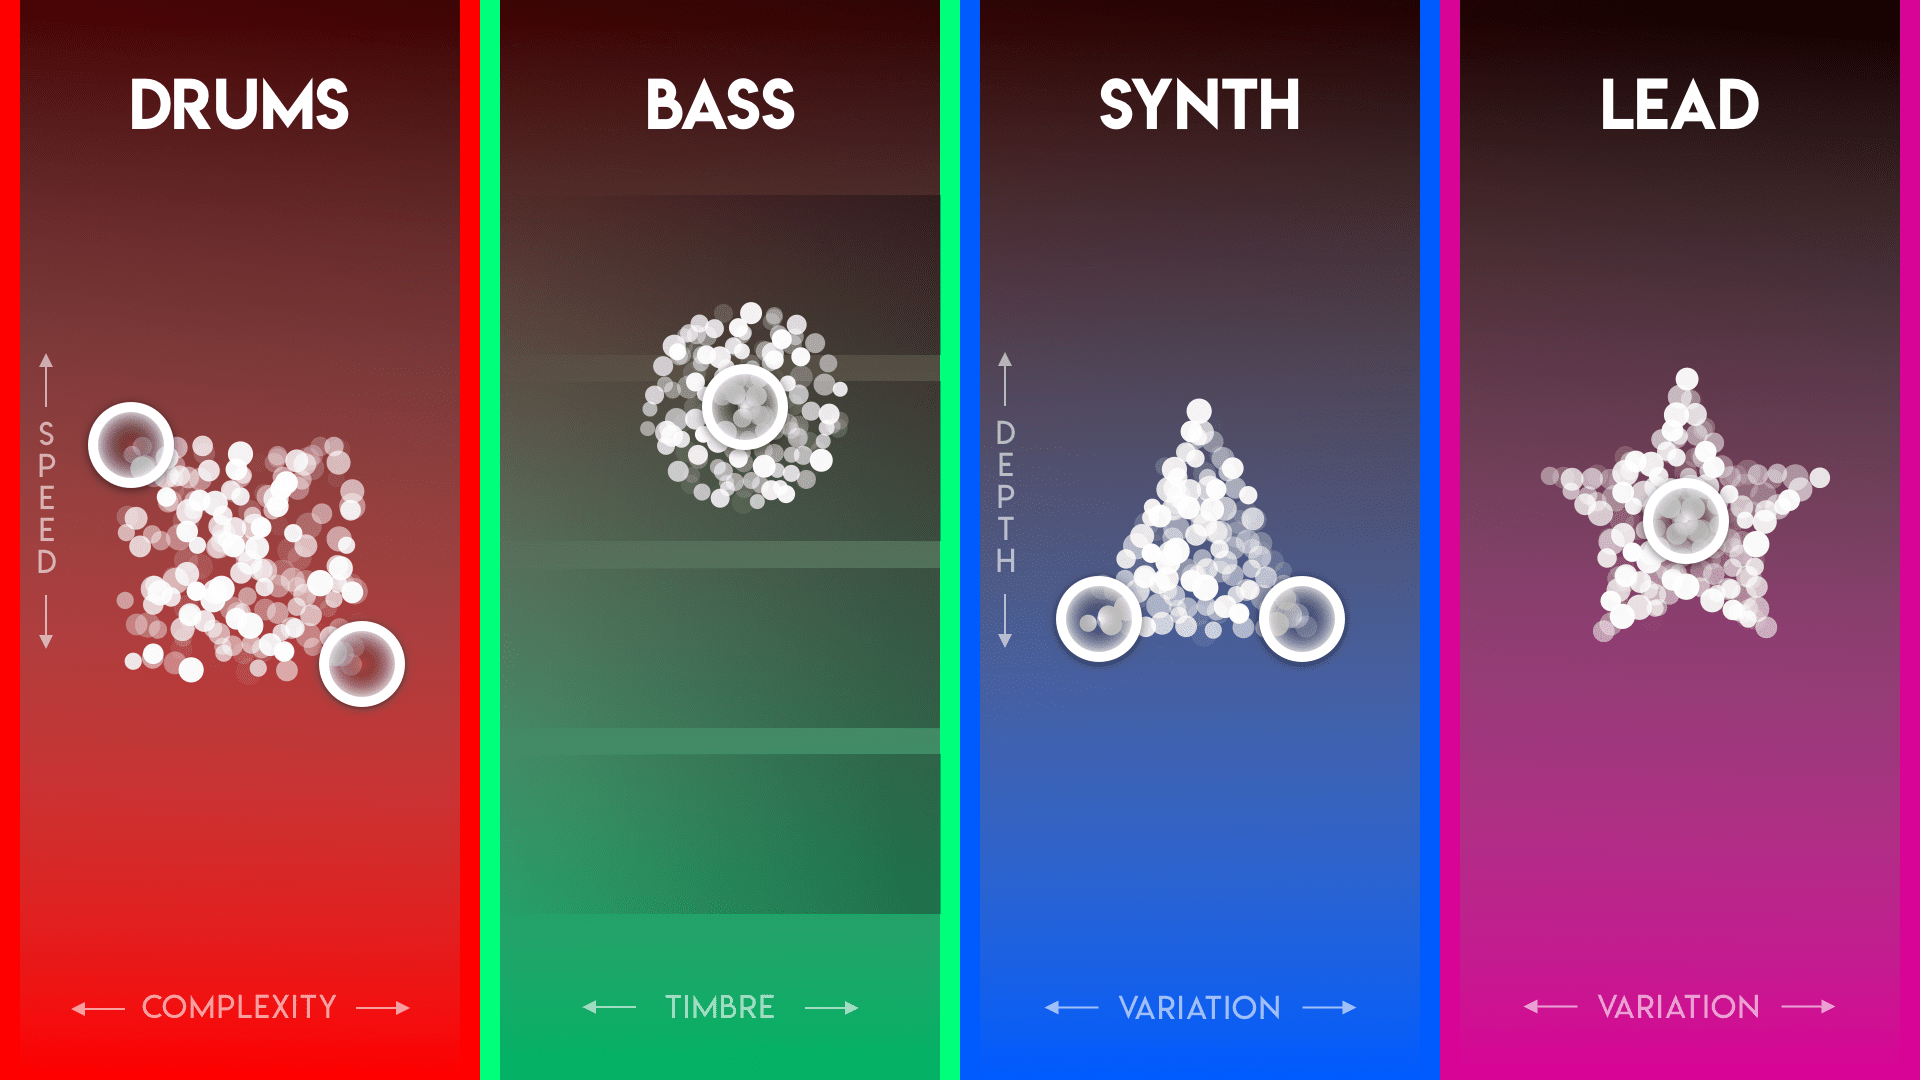
\includegraphics[width=0.90\textwidth]{UI_Mockup.png}}
    \caption{Mockup: User interface}
    \label{fig:Mockup}
\end{figure}

\subsection{Placement and movement}

These shapes could either be place in a dedicated place on a screen, which corresponds to the physical location of the user in relation to the other users.
But its also possible to make the shapes mixing and moving around each other. This might create an issue since the movement isn't closely related to musical parameters.
However, the latter solution is the visually more pleasing one. This has to be determined by simple testing.

The hue however should always correspond to a marked area on the floor. By doing so, the user will be able to quickly determine his corresponding shape.
The saturation of the hue could be used to represent certain states.

\end{document}